\subsection{Who is Who?}

\begin{frame}{\myframetitle}
	\begin{fancycolumns}
		\begin{example}{Who Are You?}
			\begin{itemize}
				\item A student in BeNeFri's \emph{Joint Master in Computer Science}, interested in
				\begin{itemize}
					\item the topics of the \emph{Distributed Software Systems} track (T2),
					\item \emph{learning} about the basic principles of systematically managing software variability,
					\item \emph{experimenting} with novel software engineering methods and tools,
					\item getting in touch with current \emph{research} on software product lines.
				\end{itemize}
			\end{itemize}
		\end{example}
	\nextcolumn
		\begin{note}{Who Are We?}
			\centering
			\parbox{0.45\linewidth}{
				\centering
				\href{https://seg.inf.unibe.ch/people/timo/}{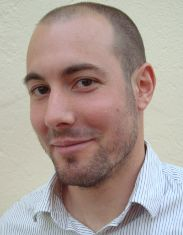
\includegraphics[width=0.9\linewidth]{timo-kehrer}}\\[.5ex]
				\href{https://seg.inf.unibe.ch/people/timo/}{\emph{Timo Kehrer}}\\[.5ex]
				\small Professor for Software Engineering \\[.5ex]
				\href{https://seg.inf.unibe.ch/}{\small \emph{SEG @ UniBE}}
			}
			\parbox{0.45\linewidth}{
				\centering
				\href{https://seg.inf.unibe.ch/people/}{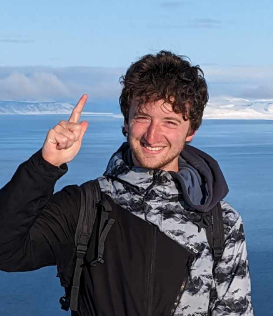
\includegraphics[width=0.9\linewidth]{roman-rmachacek}}\\[.5ex]
				\href{https://seg.inf.unibe.ch/people/}{\emph{Roman Macháček}}\\[.5ex]
				\small PhD Student with research interests in SPLs \\[.5ex]
				\href{https://seg.inf.unibe.ch/}{\small \emph{SEG @ UniBE}}
			}
		\end{note}
	\end{fancycolumns}
\end{frame}

\subsection{Where and When?}

\begin{frame}{\myframetitle}
	\begin{fancycolumns}
		\begin{definition}{Lecture}
			\begin{itemize}
				\item once per week
				\begin{itemize}
					\item on \emph{Tuesday}, 14:15--16:00
					\item Hörsaal 002, Engehalde, E8 (UniBE)
					\item starts on Tuesday, September 17, 2024
				\end{itemize}
				\item usually held by Timo
				\item \emph{slides} are available on \href{https://ilias.unibe.ch/ilias.php?baseClass=ilrepositorygui&cmd=infoScreenGoto&ref_id=3112374}{ILIAS}
				\item lectures are meant to be \emph{interactive}, you are kindly invited to \emph{actively participate}!
				\item guest lecture (research talk) planned on December 10
				%\begin{itemize}
					%\item industry talk around Christmas
					%\item research talk at end of January
				%\end{itemize}
			\end{itemize}
		\end{definition}
	\nextcolumn
		\begin{example}{Exercise}
			\begin{itemize}
				\item once per week 
				\begin{itemize}
					\item on \emph{Tuesday}, 16:15--17:00
					\item Hörsaal 002, Engehalde, E8 (UniBE)
					\item starts on Tuesday, September 17, 2024
				\end{itemize}
				\item usually held by Roman
				\item \emph{exercises} are available on \href{https://ilias.unibe.ch/ilias.php?baseClass=ilrepositorygui&cmd=infoScreenGoto&ref_id=3112374}{ILIAS}
				\item typically 2 weeks time to work on \emph{practical tasks}
				%\item lab exercise planned for end of January
			\end{itemize}
		\end{example}
	\end{fancycolumns}
\end{frame}

\subsection{Taking the Exam, and Then?}

\begin{frame}{\myframetitle}
	\begin{fancycolumns}
		%\begin{note}{Exam Eligibility \deutsch{Prüfungszulassung}}
			%\begin{itemize}
				%\item 60\% of all normal tasks \deutsch{Votierungspunkte}
				%\item 70\% for Master students
				%\item 3 presentation points \deutsch{Vortragspunkte}
				%\item all practical tasks (in teams of 2--3 students)
			%\end{itemize}
		%\end{note}
		\begin{definition}{Exam}
			\begin{itemize}
				\item \emph{oral exam} ($\approx 20$ minutes)
				\item 1--2 exam days in January (details will follow)
				\item \emph{Course registration through Academia until October 11, 2024}!
				\item \emph{Exam registration through Academia until January 3, 2025}!
			\end{itemize}
		\end{definition}
	\nextcolumn
		\begin{example}{Further Studies}
			\begin{itemize}
				\item \emph{Seminar Software Engineering} (offered every semester)
				\item \emph{Master Thesis} (several open topics on SPLE)
				\item \emph{PhD Thesis?} (SPLs are still actively researched)
			\end{itemize}
			\ldots{} Just contact us and let us know \ldots
		\end{example}
	\end{fancycolumns}
\end{frame}
